\IEEEraisesectionheading{\section{Introduction}\label{sec:introduction}}

Humans are faced with a stream of high-dimensional sensory inputs and minimal external supervision, and yet, remarkably, are able to learn a range of complex yet generalizable concepts and behaviors.
While there has been significant progress in developing deep reinforcement learning algorithms that learn complex skills and scale to high-dimensional observation spaces, such as pixels~\cite{tdgammon,atari,e2e,alphago}, learning behaviors that \emph{generalize} to new objects, goals, or scenes remains an open problem.
The key to generalization is diversity. When deployed in a narrow, closed-world environment, a reinforcement learning algorithm will recover skills that are successful only in a narrow range of settings. 
Learning skills in diverse, open-world environments, such as the real world, presents a number of significant challenges: external reward feedback is extremely sparse or non-existent, and the agent has only indirect access to the state of the world through its senses which, in the case of a robot, might correspond to cameras and joint encoders.

\begin{figure}[t]
	\centering
	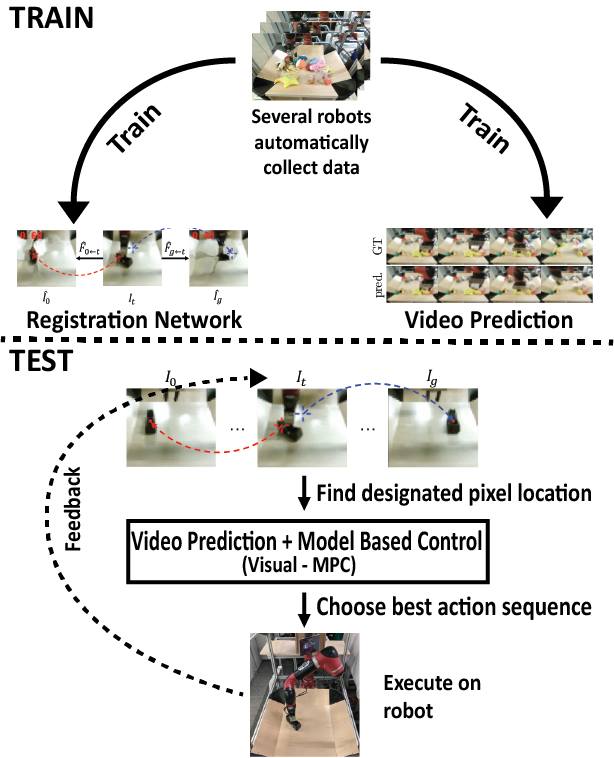
\includegraphics[width=.8\columnwidth,trim={3.2mm 0 0 0},clip]{images_general/new_overview.png}
	\caption{\small{\todo{Example Trajectories for different tasks, solved by Visual MPC}}}
	\label{fig:example_traj}
\end{figure}

We approach the problem of learning generalizable behavior in the real world from the standpoint of sensory prediction. Prediction is often considered a fundamental component of intelligence, and, crucially, prediction of raw sensory observations does not make any assumptions about the availability of state information or extrinsic reward feedback. Learning via prediction is possible directly from a stream of raw sensory observations, such as images from a camera. These observations are both information-rich and high-dimensional, presenting both an opportunity and a challenge. Future observations provide a substantial amount of supervisory information for a machine learning algorithm. However, the predictive model must have the capacity to predict these high-dimensional observations, and the control algorithm must be able to use such a model to effectively select actions to accomplish user-specified goals.



%Instead of focusing on mastery of highly-specialized skills in closed-world environments, here we focus on \emph{generalization} in diverse environments.
%%SL.09.03: this is an important and critical sentence, but I don't like that we from the outset present it in contrast to something so negative (those other guys fail at this, but we don't) -- just say what we do well, and then talk about alternatives. I think we can motivate the work and explain the challenge without necessarily getting so bogged down in the failure of prior work.
To study \emph{generalization} in reinforcement learning, we must enable our model to learn from a diverse range of interactions with varied objects. We therefore consider a minimally structured robotic control domain, where data is collected by the robot via unsupervised interaction with a wide range of objects. The robot collects a stream of raw sensory observations (image pixels), without any reward signal at training time, and without the ability to reset the environment between episodes. This setting is both realistic and, in order to study learning in diverse settings, necessary in order to enable and automated and unattended collection of diverse interaction experience. Since the training setting affords no readily accessible reward signal, learning by prediction presents an appealing option: the supervision signal for prediction is always available even in the stream of unsupervised experience, and a predictive model can be used at test time to perform new tasks without additional learning.
We therefore propose to learn action-conditioned predictive models directly on raw pixel observations, and show that they can be used to accomplish manipulation tasks on a real robot in the physical world at test-time.
Sensory prediction models are goal-agnostic, which enables learning for a variety of different goals at the same time. By learning from raw sensor readings, they are also fully general, in that they do not require access to any other state representation beyond the observations.
Our overall approach amounts to a deep model-based reinforcement learning algorithm that leverages video prediction models to perform a variety of pixel-based control tasks.

%In addition the practicality of leveraging the only available supervision in such sparse reward environments, sensory prediciton models are also goal-agnostic, which enables learning for a variety of different goals.
%% TODO - motivate why not to learn a model on top of a more abstract representation of the observations? [The supervision, inherently, comes from the same place.]
%TODO - motivate why raw pixels rather than more compact representation (because pixels contain complete information -- can give Sergey's crossing-the-street example -- and pixels are the only thing that is readily available; also pixels contain more supervision)

\begin{figure}[t]
\centering
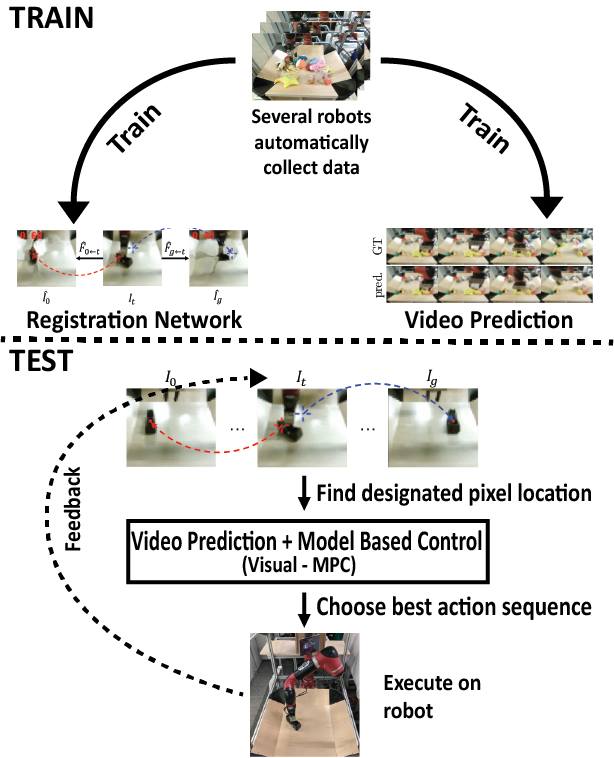
\includegraphics[width=.8\columnwidth,trim={3.2mm 0 0 0},clip]{images_general/new_overview.png}
\caption{\small{\todo{Overview of visual MPC concept}}}
\label{fig:overview}
\end{figure}
%%SL.10.15: It doesn't appear that this figure is referenced anywhere or used.

%Despite the benefits, a number of challenges arise when aiming to use sensory prediction models: how can we learn a model of high-dimensional observations, and how should an objective or reward be determined with respect to the predicted observations? %how should experience be collected? %how should actions be chosen with respect to the model?
%We discuss each of these design decisions and propose several options, weighting the benefits and trade-offs of each.
%%SL.09.03: sounds a bit too much like a laundry list, can we pull some broader themes and dive into details later?
%Our overall approach amounts to a deep model-based reinforcement learning algorithm that leverages video prediction models to achieve a variety of pixel-based control tasks without shaped reward information.

The main contributions of this work are as follows. We present visual MPC, a general framework for deep reinforcement learning with sensory prediction models that is suitable for learning behaviors in diverse, open-world environments.
We describe deep network architectures that are effective for predicting pixel-level observations amid occlusions and with novel objects. Unlike low-dimensional representations of state, specifying and evaluating the reward from pixel predictions at test-time is nontrivial, and we present several practical methods for specifying and evaluating progress towards the goal---including distances to goal pixel positions, registration to goal images, and image classifiers---and compare their effectiveness and use-cases.
%, abstracting away the model architecture %, the policy optimization, 
%and the form of the reward function with respect to predicted observations.
%%SL.09.03: seems reasonable, but when we abstract away so much, we just get the classic model-based RL problem setting. Maybe this is a little bit too much abstraction.
%We then propose model architectures for prediction that can better maintain object permanence through occlusions via temporal skip connections. 
%To handle the challenge of evaluating progress towards the goal from pixel-level predictions, we present several forms of reward specification and evaluation,
%%SL.09.03: I wouldn't put this "Second" -- maybe something more general like architectures for prediction?
%Third, we discuss several forms of planning objectives, 
%including goal pixel positions, goal image registration, and image classifiers.
%%SL.09.03: without motivation, this seems a bit arbitrary. I think this is a good contribution, but the phrasing makes it seem like a less significant detail somehow.
Finally, our evaluation shows how these components can be combined to enable a real robot to perform a range of object manipulation tasks from raw pixel observations. Our experiments include manipulation of previously unseen objects, handling multiple objects, pushing objects around obstructions, handling clutter, manipulating deformable objects such as cloth, recovering from large perturbations, and grasping and maneuvering objects to user-specified locations in 3D-space. These results represent a significant advance in the \emph{generality} of skills that can be acquired by a real robot operating on raw pixel values.

This article combines and extends material from several prior conference papers~\cite{foresight,sna,ebert2018robustness,flo}, presenting them in the context of a unified system. We include additional experiments, including cloth manipulation and placing tasks, analysis of each method involving XX, as well as a comprehensive, open-sourced simulation environment to facilitate future research and better reproducibility.
%%SL.10.15: make sure we actually have all this :)


\todo{make big VMPC diagramm!!}



 





